\documentclass{article}
\usepackage{amsmath, amssymb, amsthm, amsfonts, bm}
\theoremstyle{remark}

\usepackage{physics}
\usepackage[a4paper, total={6in,10in}]{geometry}
\usepackage[dvipsnames]{xcolor}
\usepackage{xcolor-material}
\usepackage{hyperref}
    \hypersetup{colorlinks=true, linkcolor=ForestGreen}
\usepackage{graphicx}
    \graphicspath{{./img/}}
\usepackage{tikz}
\usepackage{ragged2e}

\usepackage{soul}
\usepackage{cancel}

\usepackage{booktabs}
\usepackage{cellspace}
\newcolumntype{L}[1]{>{\centering\arraybackslash}m{#1}}  % cell with auto-wrap, e.g. |L{0.2\linewidth}|L{0.8\linewidth}|
\usepackage{makecell}  % use Sc instead of c
\setlength{\cellspacetoplimit}{10pt}
\setlength{\cellspacebottomlimit}{10pt}

\newcommand{\where}[1]{\begin{flushright}where #1.\end{flushright}}
\newcommand{\wher}[1]{\begin{flushright}#1.\end{flushright}}
\newcommand{\mylabel}[2]{\hyperref[#1]{#2}\label{back:#1}}
\newcommand{\myref}[1]{\hyperref[back:#1]{$\bigstar$}\label{#1}}
\newcommand{\e}{\hat{\vb{e}}}  % unit vector
\newcommand{\s}[1]{\textsubscript{#1}}
\newcommand{\ppdv}[4][]{\left(\pdv[#1]{#2}{#3}\right)_{#4}}
\everymath{\displaystyle}
\begin{document}

\title{Cheatsheet}
\date{}
\maketitle

\subsubsection*{1}
\begin{enumerate}
    \item \begin{align*}
        \div\vb{D}=\rho\\
        \curl\vb{E}=-\vb{\dot B}\\
        \div\vb{B}=0\\
        \curl\vb{H}=\textcolor{red}{\vb{J}+\vb{\dot D}}
    \end{align*}
    \item $\vb{F}=q\vb{E}+q\vb{v}\times\vb{B}$
    \item \begin{itemize}
        \item $\vb{p} = q\vb{a} $
        \item $\vb{m} = I\int_S\dd\vb{S}$
        \item $\vb{G} = \vb{p}\times\vb{E} $, $\vb{G} = \vb{m}\times\vb{B} $
        \item $U=-\vb{p}\cdot\vb{E}$, $U=-\vb{m}\cdot\vb{B}$
        \item $\vb{F} = -\grad U(\vb{r})$, $\vb{F} = (\vb{p}\cdot\grad)\vb{E}$, $\vb{F}=(\vb{m}\cdot\grad)\vb{B}$
    \end{itemize}
    \item $U_E = \frac{1}{2}\epsilon\epsilon_0|\vb{E}(\vb{r})|^2 = \frac{1}{2}\vb{D}(\vb{r})\cdot\vb{E}(\vb{r}) $\\
        $U_B = \frac{1}{2}\vb{B}(\vb{r})\cdot\vb{H}(\vb{r})$
    \item $\vb{D} = \epsilon_0\vb{E}+\vb{P} = \epsilon_0(1+\chi)\vb{E} $, $\vb{B}=\mu_0(\vb{H}+\vb{M})=\mu_0(1+\chi_m)\vb{H}$
    \item $\boxed{\curl(\curl\vb{F})=\grad(\div\vb{F})-\laplacian{\vb{F}}}$\begin{itemize}
            \item $\dd\vb{B} = \frac{\mu_0 I}{4\pi R^2}\dd\vb{l}\times\vb{\hat R}$
            \item $\laplacian\vb{E}=\mu_0\epsilon_0\pdv[2]{\vb{E}}{t}\\
                    \laplacian\vb{H}=\mu_0\epsilon_0\pdv[2]{\vb{H}}{t}$ (No charge, no current)\\
                    $\frac{E_x}{B_y}=\frac{\omega}{k}=v=\frac{1}{\sqrt{\epsilon\epsilon_0\mu\mu_0}}\\
                        \frac{E_x}{H_y}=Z=\sqrt{\frac{\mu\mu_0}{\epsilon\epsilon_0}}$\\
                    $\vb{N}=\vb{E}\times\vb{H}$\\
                    $\vb{R}=\frac{\vb{N}}{c}$
        \end{itemize}
    \item $\vb{m}=V\vb{M}=I\int\dd S$
    \item Scalar potential $\vb{B}=\mu_0\vb{H}=-\mu_0\grad\vb{\phi}_m$, vector potential $\vb{B}=\curl\vb{A}, \div\vb{A}=0, -\laplacian{\vb{A}}=\mu_0\vb{J}$
    \item $Z=\frac{V}{I}=\sqrt{\frac{L}{C}}$
    \item $r=\frac{V_r}{V_i}=\frac{Z_t-Z}{Z_t+Z}$, $t=\frac{V_t}{V_i}=\frac{2Z_t}{Z_t+Z}$
\end{enumerate}

\subsubsection*{2}
\begin{enumerate}
    \item $\vb{J}=\sum\vb{r}\times\vb{p}=\sum\vb{r}\times m(\bm{\omega}\times\vb{r})=\textcolor{red}{\sum m(r^2\bm{\omega}-\vb{r}(\vb{r}\cdot\bm{\omega}))} = \sum m(\bm{r}^T\bm{r}\bm{1}-\bm{r}\bm{r}^T)\bm{\omega} = \bm{I}\bm{\omega} = \begin{pmatrix}
        \textstyle\sum m(y^2+z^2) & -\textstyle\sum mxy & -\textstyle\sum mxz\\
        -\textstyle\sum mxy & \textstyle\sum m(x^2+z^2) & -\textstyle\sum myz\\
        -\textstyle\sum mxz & -\textstyle\sum myz & \textstyle\sum m(x^2+y^2)\\
    \end{pmatrix}\bm{\omega} $
    \item For body frame $S$, $\bm{G}=\left[\dv{\bm{J}}{t}\right]_S+\bm{\omega}\times\bm{J}$, Euler's equations are \begin{align*}
        G_1 = I_1\dot\omega_1 + (I_3-I_2)\omega_2\omega_3\\
        G_2 = I_2\dot\omega_2 + (I_1-I_3)\omega_3\omega_1\\
        G_3 = I_3\dot\omega_3 + (I_2-I_1)\omega_1\omega_2
    \end{align*}
    
    (Because $\bm{J}=I\bm{\omega} = \sum_{i=1}^{3} I_i\omega_i\hat{e}_i$, $\bm{G}=\sum_{i=1}^{3} I_i\dot\omega_i\hat{e}_i+I_i\omega_i\dv{\hat{e}_i}{t}$ and $\boxed{\dv{\hat{e}_i}{t}=\bm{\omega}\times\hat{e}_i}$)
    \item $T = \frac{1}{2}\sum m(\bm{\omega}\times\bm{r})\cdot(\bm{\omega}\times\bm{r}) = \frac{1}{2}\sum m\bm{\omega}\cdot(\bm{r}\times(\bm{\omega}\times\bm{r})) = \frac{1}{2}\bm{\omega}\cdot\bm{J} = \frac{1}{2}\bm{\omega}^T I\bm{\omega}$
    \item $\Omega_b\equiv\frac{I_1-I_3}{I_1}\omega_3$
    \item $\Omega_s=\frac{\dot\omega_1}{|\bm{\omega}|\sin\theta_s}=\frac{J}{I_1}$
    \item $\Omega_b\sin\theta_b=\Omega_s\sin\theta_s$ (Poinsot)
    \item Symmetric top with Euler angles $(\theta,\phi,\chi)$
    
    \begin{minipage}[b]{0.6\textwidth}
        \centering
        \begin{itemize}
            \item $\bm{\omega}=\dot\phi\hat{e}_z+\dot\theta\hat{e}_1+\dot\chi\hat{e}_3$
            \item In body frame $S$, $\bm{\omega}=(\dot\theta,\dot\phi\sin\theta,\dot\chi+\dot\phi\cos\theta)$
            
            $\bm{J}=(I_1\dot\theta,I_1\dot\phi\sin\theta,I_3(\dot\chi+\dot\phi\cos\theta))$
            \item Keep $\omega_3=\dot\chi+\dot\phi\cos\theta$, $J_z=J_3\cos\theta+J_2\sin\theta$ constant
            \item We get $\dot\phi=\Omega_s$, $\dot\chi=\Omega_b$
        \end{itemize}
    \end{minipage}
    \hfill
    \begin{minipage}[b]{0.39\textwidth}
        \centering
        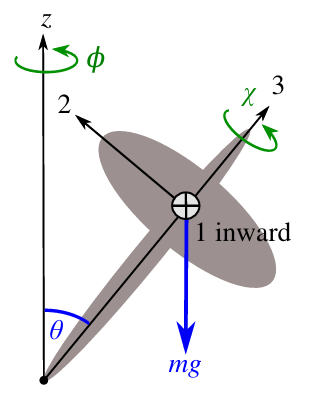
\includegraphics[width=0.4\linewidth]{Lagrange's approach.png}
    \end{minipage}
    \item For simplicity, only consider principal axis to express $e$ and $\tau$ as vectors
    \item Strain is $e=\delta l/l$, stress is $\tau=-P=-F/A$, for isotropic material, $\textstyle E\vb{e}=\begin{pmatrix}
        1 & -\sigma & -\sigma\\
        -\sigma & 1 & -\sigma\\
        -\sigma & -\sigma & 1
    \end{pmatrix}\bm{\tau}$, $\sigma$ is Poisson ratio, $e_1=e_2=e_3=\frac{\tau(1-2\sigma)}{E}$, $\frac{\delta V}{V}\approx e_1+e_2+e_3 = \frac{3\tau(1-2\sigma)}{E}$, $\boxed{B=\frac{E}{3(1-2\sigma)}}$
    \item $\bm{\tau}=\begin{pmatrix}
        1 & -\sigma & -\sigma\\-\sigma & 1 & -\sigma\\-\sigma & -\sigma & 1\end{pmatrix}^{-1}
        E\vb{e} = \frac{E}{(\sigma+1)(1-2\sigma)}\begin{pmatrix}
            1-\sigma & \sigma & \sigma\\
            \sigma & 1-\sigma & \sigma\\
            \sigma & \sigma & 1-\sigma\\
        \end{pmatrix}\vb{e} = \lambda(e_1+e_2+e_3)+2G\bm{e} = \lambda\Tr(\bm{e})\bm{I}+2G\bm{e}$, Lam\'e's constant $\boxed{\lambda\equiv\frac{E\sigma}{(1+\sigma)(1-2\sigma)}, G=\frac{E}{2(1+\sigma)}}$, $\lambda=B-\frac{2}{3}G$    
    \item $W=-\dv{F}{x},F=-\dv{B}{x},B=\frac{EI}{R}=EIy''=\int y\cdot\tau\dd A$, $\tau=Ee=E\frac{y}{R}$, $I=\int y^2\textcolor{red}{\dd A}$
    \item $\frac{D\vb{v}}{D t}=\pdv{\vb{v}}{t}+\vb{v}\cdot\grad\vb{v}$
    \item $\rho\frac{D\vb{v}}{D t}=-\grad P+\rho\vb{g}+\eta\laplacian{\vb{v}}$ ($\eta=0$, Euler's equation)
    \item $P+\frac{1}{2}\rho v^2+\rho\phi=C$
    \item $\Phi=v_0\cos\theta\left(r+\frac{a^3}{2r^2}\right)$
    \item Magnus effect $\vb{F}=\rho \vb{v}\times\textbf{\kappa}$, $\kappa=2\pi r v_\theta$ is circulation around cylinder
    \item Coriolis force $2m\omega v\sin\theta$
\end{enumerate}


\subsubsection*{Examples to memorize}
\begin{enumerate}
    \item Plasma\begin{itemize}
        \item Electron $m_e\dv[2]{\vb{r}}{t}=-e(\vb{E}+\vb{v}\times\vb{B})$
        \item $B_y=E_x/c$, $c\ll|\vb{v}|$, $\vb{B}$ \textcolor{red}{ignored}
        \item $\vb{r}=\frac{e}{m_e\omega^2}\vb{E_0}e^{i(kz-\omega t)}$
        \item Electron and lattice - dipole $\vb{p}=-e\vb{r}=-\frac{e^2}{m_e\omega^2}\vb{E_0}e^{i(kz-\omega t)}$
        \item Dipole moment per unit volume $\vb{P}=-\frac{Ne^2}{m_e\omega^2}\vb{E}=\epsilon_0\chi\vb{E}$
        \item $\epsilon=1+\chi=1-\frac{Ne^2}{m_e\epsilon_0\omega^2}=\boxed{1-\frac{\textcolor{red}{\omega_p}^2}{\omega^2}}$, $\omega_p=\sqrt{\frac{N}{m_e\epsilon_0}}e$
        \item Below $\omega_p$, $\epsilon<0$, $n$ is imaginary, reflect
    \end{itemize}
    \item Conductor\begin{itemize}
        \item Currents form $\textcolor{red}{\vb{J}}=\sigma\vb{E}$, $\sigma\sim10^7\gg1$
        \item $\textcolor{red}{\curl\vb{H}}=\vb{J}+\vb{\dot D}=\sigma\vb{E}+\epsilon\epsilon_0\pdv{\vb{E}}{t}=(\sigma-i\omega\epsilon\epsilon_0)\vb{E}=-i\omega\textcolor{red}{\epsilon'}\epsilon_0\vb{E}$
        \item Effective dielectric constant $\epsilon'=\epsilon-\frac{\sigma}{i\omega\epsilon_0}\approx \boxed{i\frac{\sigma}{\omega\epsilon_0}}$
        \item $n=\sqrt{\epsilon'\mu}=\pm\frac{1+i}{\sqrt{2}}\sqrt{\frac{\sigma\mu}{\omega\epsilon_0}}$
        \item $E=E_0e^{i(\omega t-kz)}$, $c/n=\frac{\omega}{k}$
        \item $k=\frac{n\omega}{c}=\frac{1+i}{\sqrt{2}}\sqrt{\sigma\mu_0\mu\omega}=\frac{1+i}{\textcolor{red}{\delta}}$, skin depth $\boxed{\delta=\sqrt{\frac{2}{\sigma\omega\mu_0\mu}}}$
        \item $E=E_0e^{-z/\delta+i(z/\delta-\omega t)}$, exponential decay wrt. skin depth $\delta$
    \end{itemize}
    \item The skin effect \begin{itemize}
        \item $\vb{E}$ along wire ($x$ direction), $\vb{J}=\sigma\vb{E}$. $z$ is radial direction
        \item $J_x(z)=J_0e^{-z/\delta+i(z/\delta-\omega t)}$
        \item Approximate $I$ at small $\delta$, $I=\int_0^\infty J_x(z)(2\pi a)\dd z=\pi aJ_0\delta(1+i)e^{-i\omega t}$
        \item $\langle I^2\rangle=(\pi aJ_0\delta)^2$
        \item $\dd P=\frac{J^2\dd A}{\sigma}$, $P=\frac{J_0^2\pi a\delta}{2\sigma}$
        \item $R=\frac{P}{\langle I^2\rangle} = \frac{P}{\langle I^2\rangle}=\frac{1}{2\pi a\delta\sigma}=\frac{1}{\sigma A'}$
        \item Skin effect: at high $\omega$, small $\delta$, \fbox{effective area=$2\pi a\delta$} (annulus of thickness of skin depth)
    \end{itemize}
    \item Input impedance is impedance measured at the input (position matters)\begin{itemize}
            \item 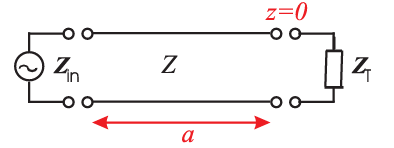
\includegraphics[width=0.5\linewidth]{input impedance.png}
            \item $V_i=V_1e^{-i(kz-\omega t)}$, $V_r=rV_1e^{-i(-kz-\omega t)}$, $\frac{V_i}{I_i}=Z$, $\frac{V_r}{I_r}=-Z$
            \item $Z_{\text{in}}=\eval{\frac{V_i+V_r}{I_i+I_r}}_{r=a}=\frac{e^{ika}+re^{-ika}}{e^{ika}-re^{-ika}}Z$, $\frac{Z_{\text{in}}}{Z}=\frac{Z_t\cos(ka)+iZ\sin(ka)}{Z\cos(ka)+iZ_t\sin(ka)}$
            \item Short-circuit, $Z_t = 0$, $\frac{Z_{\text{in}}}{Z}=i\tan(ka)$
            \item Open-circuit, $Z_t\rightarrow\infty$, $\frac{Z_{\text{in}}}{Z}=-i\cot(ka)$
            \item Quater-wavelength, $a=\lambda/4, ka=\pi/2$, $\frac{Z_{\text{in}}}{Z}=\frac{Z}{Z_t}$
        \end{itemize}
    \item (Non-TEM) Parallel plate waveguide \begin{itemize}
            \item \includegraphics*[width=0.5\linewidth]{waveguide.png}
            \item $k^2=k_x^2+k_z^2$, $k_z=k_g$, $k_x=\frac{m\pi}{a}$ (standing wave)
        \end{itemize}
    \item Rectangular waveguide\begin{itemize}
            \item General $TE_{mn}$, transverse electric, $n$ and $m$ in x,y direction
            \item $(k_x,k_y,k_z)=\left(\frac{m\pi}{a},\frac{n\pi}{b},k_g\right)$
            \item \begin{align*}
                    E_x &= A_0k_y\cos(k_x x)\sin(k_y y)\cos(k_z z-\omega t)\\
                    E_x &= -A_0k_y\sin(k_x x)\cos(k_y y)\cos(k_z z-\omega t)\\
                    E_z&=0
                \end{align*}
            \item $\frac{\omega^2}{c^2}=k_x^2+k_y^2+k_z^2$
            \item $k_z=k_g$, if imaginary, evanescent
            \item \includegraphics*[width=\linewidth]{rect_waveguide.png}
        \end{itemize}
\end{enumerate}

\end{document}